\section{Experiments on Feature Inversion}
\label{sec:experimental}

\begin{table}[t]
\vspace{0.3 cm}
\small
\def\arraystretch{1.25}
\setlength\tabcolsep{4pt}
\begin{center}
\fontsize{7}{7}\selectfont
\caption{\label{tab:inversion_alexnet}AlexNet feature inversion on ImageNet. Under distinct training losses, inverting AR features via our proposed generator is consistently more accurate than inverting standard features.}
\vspace{0.1cm}
\begin{tabular}{c|c|c|c|c} 
\specialrule{.15em}{.05em}{.05em} 
Losses & Model & PSNR (dB)$\uparrow$ & SSIM$\uparrow$ & LPIPS$\downarrow$\\
\hline
 \multirow{2}{*}{\makecell{Pixel}} & \makecell{Standard} & $17.562\pm 2.564$ & $0.454\pm 0.167$ & $0.624\pm 0.099$\\
 & \makecell{AR (ours)} & $\mathbf{19.904\pm 2.892}$ & $\mathbf{0.505\pm 0.169}$ & $\mathbf{0.596\pm 0.104}$\\
 \hline
 \multirow{2}{*}{\makecell{Pixel, Feature}} & \makecell{Standard} & $14.462\pm 1.884$ & $0.103\pm 0.044$ & $0.713\pm 0.046$\\
 & \makecell{AR (ours)} & $\mathbf{17.182\pm 2.661}$ & $\mathbf{0.284\pm 0.111}$ & $\mathbf{0.601\pm 0.034}$\\  
 \hline
 \multirow{2}{*}{\makecell{Pixel, Feature,\\GAN}} & \makecell{Standard} & $15.057\pm 2.392$ & $0.307 \pm 0.158$ & $\mathbf{0.547\pm 0.055}$\\
 & \makecell{AR (ours)} & $\mathbf{17.227\pm 2.725}$ & $\mathbf{0.358\pm 0.163}$ & $0.567\pm 0.056$\\
\specialrule{.15em}{.05em}{.05em} 
\end{tabular}
\end{center}
\vspace{-0.4 cm}
\end{table}

\begin{figure}[t]
\centering
\begin{minipage}[t]{0.1429\textwidth}
\centering \colorbox{white}{\textbf{\scalebox{.8}{G. truth}}}
\end{minipage}\begin{minipage}[t]{0.1429\textwidth}
\centering \colorbox{white}{\textbf{\scalebox{.8}{Standard}}}
\end{minipage}\begin{minipage}[t]{0.1429\textwidth}
\centering \colorbox{white}{\textbf{\scalebox{.8}{AR (ours)}}}
\end{minipage}\begin{minipage}[t]{0.1429\textwidth}
\centering \colorbox{white}{\textbf{\scalebox{.8}{Standard}}}
\end{minipage}\begin{minipage}[t]{0.1428\textwidth}
\centering \colorbox{white}{\textbf{\scalebox{.8}{AR (ours)}}}
\end{minipage}\begin{minipage}[t]{0.1429\textwidth}
\centering \colorbox{white}{\textbf{\scalebox{.8}{Standard}}}
\end{minipage}\begin{minipage}[t]{0.1429\textwidth}
\centering \colorbox{white}{\textbf{\scalebox{.8}{AR (ours)}}}
\end{minipage}\vspace{-0.4\baselineskip}

\begin{minipage}{0.1429\textwidth}
\centering\textbf{ }
\end{minipage}\begin{minipage}[t]{0.1429\textwidth}
\centering \scalebox{0.65}{Pix.}
\end{minipage}\begin{minipage}[t]{0.1429\textwidth}
\centering \scalebox{0.65}{Pix.}
\end{minipage}\begin{minipage}[t]{0.1429\textwidth}
\centering \scalebox{0.65}{Pix., Feat.}
\end{minipage}\begin{minipage}[t]{0.1428\textwidth}
\centering \scalebox{0.65}{Pix., Feat.}
\end{minipage}\begin{minipage}[t]{0.1429\textwidth}
\centering \scalebox{0.65}{Pix., Feat., GAN}
\end{minipage}\begin{minipage}[t]{0.1429\textwidth}
\centering \scalebox{0.65}{Pix., Feat., GAN}
\end{minipage}

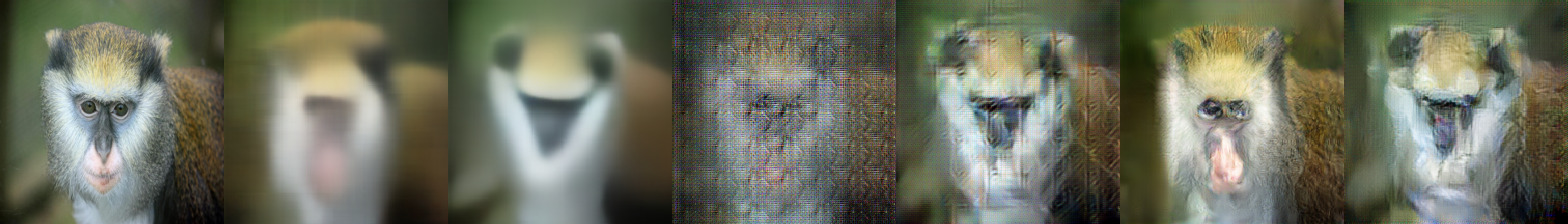
\includegraphics[width=\textwidth]{figs/ablation/ablation_tile2.jpg}

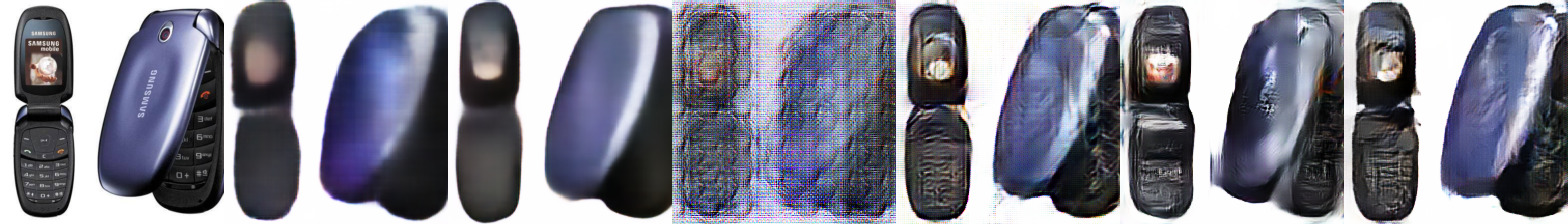
\includegraphics[width=\textwidth]{figs/ablation/ablation_tile9.jpg}

\caption{\label{fig:inversion_alexnet}AlexNet feature inversion on ImageNet. \layer{Conv5} features are inverted using our proposed generator under three different training criteria. Reconstructions from AR features are more faithful to the ground-truth image.}
\vspace{-0.4cm}
\end{figure}


We begin analyzing the reconstruction accuracy achieved by inverting features from different classifiers and empirically show that learning how to invert AR features via our proposed generator improves over standard feature inversion. Refer to \secref{sec:supp_results} and \secref{sec:supp_proposed_method} for additional inversion results and training details.

\subsection{Reconstruction Accuracy of AR Autoencoders}
\label{sec:experimental_inverting}
\textbf{Inverting AlexNet features.} Standard and AR AlexNet autoencoders are trained as described in \secref{sec:proposed_inversion} on ImageNet for comparison purposes. The AR AlexNet classifier is trained via $\ell_{2}$-PGD attacks \cite{madry_2018_towards} of radius $\varepsilon=\frac{3}{255}$ and $7$ steps of size $0.5$. Training is performed using $90$ epochs via SGD with a learning rate of $0.1$ reduced $10$ times every $30$ epochs. On the other hand, the standard AlexNet classifier is trained on natural images via cross-entropy (CE) loss with the same SGD setup as in the AR case.

Next, generators are trained  using pixel, feature and GAN losses to invert AlexNet \layer{conv5} features (size $6\times6\times256$). Both AR and standard models use the same generator architecture, which corresponds to the mirror network of the encoder. We deliberately use a simple architecture to highlight the reconstruction improvement is due to inverting AR features and not the generator capacity. We also train generators using (i) pixel and (ii) pixel and feature losses to ablate their effect. Reconstruction quality is evaluated using PSNR, SSIM and LPIPS.

Under all three loss combinations, reconstructions from AR AlexNet features obtain better PSNR and SSIM than their standard counterparts (\tabref{tab:inversion_alexnet}). Specifically, inverting AR AlexNet features gives an average PSNR improvement of over $2$ dB in all three cases. LPIPS scores also improve, except when using pixel, feature and GAN losses. Nevertheless, inverting AR features obtain a strong PSNR and SSIM improvement in this case as well. Qualitatively, inverting AR features better preserves the natural appearance in all cases, reducing the checkerboard effect and retaining sharp edges (\figref{fig:inversion_alexnet}).

\textbf{Inverting VGG features.} We extend the analysis to VGG-16 trained on ImageNet-143 and evaluate the reconstruction improvement achieved by inverting its AR features. We use the AR pre-trained classifier from the recent work by Liu et al.~\cite{liu_2018_adv} trained using $\ell_{\infty}$-PGD attacks of radius $\varepsilon=0.01$ and $10$ steps of size $\frac{1}{50}$. Training is performed using $80$ epochs via SGD with a learning rate of $0.1$ reduced $10$ times every $30$, $20$, $20$ and $10$ epochs. On the other hand, its standard version is trained on natural images via CE loss with the same SGD setup as in the AR case.

Generators are trained on pixel and feature losses to invert VGG-16 \layer{conv5\_1} features (size $14 \times 14 \times 512$). Similarly to the AlexNet analysis, generators inverting both standard and AR features correspond to the mirror network of the encoder. We evaluate the reconstruction accuracy of both models and report their level of adversarial robustness (\tabref{tab:inversion_vgg16} and \figref{fig:inversion_vgg16}).

\begin{table}[t]

\centering
\begin{minipage}{0.575\textwidth}
\fontsize{8.45}{10.45}\selectfont
\begin{center}
\vspace{-0.8 cm}
\caption{\label{tab:inversion_vgg16} AR VGG-16 \cite{liu_2018_adv} feature inversion on ImageNet. Training our generator via pixel and feature losses, reconstruction largely improves by inverting AR representations.}
\begin{tabular}{c|c|c}
\specialrule{.15em}{.05em}{.05em} 
 & Standard Model & AR Model (ours)\\
 \hline
\makecell{Standard Accuracy} & $65.0$ & $48.7$\\
\makecell{$\ell_{\infty}$ PGD Accuracy} & $0$ & $23.0$\\
\hline
\makecell{PSNR (dB) $\uparrow$} & $18.35\pm 2.471$ & $\mathbf{21.063\pm 3.132}$\\
\makecell{SSIM $\uparrow$} & $0.466\pm 0.2$ & $\mathbf{0.538\pm 0.165}$\\
\makecell{LPIPS $\downarrow$} & $0.327\pm 0.101$ & $\mathbf{0.225\pm0.057}$\\
\specialrule{.15em}{.05em}{.05em} 
\end{tabular}
\end{center}
\end{minipage}
\hfill
\begin{minipage}{0.375\textwidth}
\hspace{2.21\baselineskip}\noindent\fcolorbox{white}{white}{\begin{minipage}[t]{0.155\textwidth}
\centering\textbf{{\scalebox{0.525}{\hspace{-0.25\baselineskip}G. truth}}}
\end{minipage}}\noindent\fcolorbox{white}{white}{\begin{minipage}[t]{0.16\textwidth}
\centering\textbf{{\scalebox{0.525}{\hspace{-0.15\baselineskip}Standard}}}
\end{minipage}}\noindent\fcolorbox{white}{white}{\begin{minipage}[t]{0.15\textwidth}
\centering\textbf{{\scalebox{0.525}{\hspace{-0.55\baselineskip}AR (Ours)}}}
\end{minipage}}

\begin{center}
\vspace{-0.475cm}
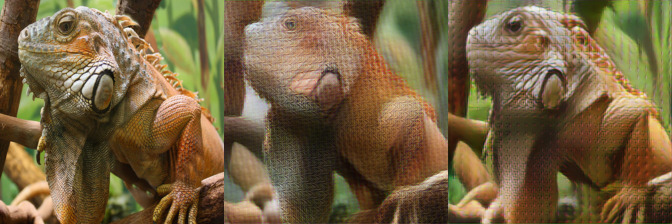
\includegraphics[width=0.63\textwidth]{figs/vgg16/rec_tile_0.jpg}


\includegraphics[width=0.63\textwidth]{figs/vgg16/rec_tile_1.jpg}


\includegraphics[width=0.63\textwidth]{figs/vgg16/rec_tile_2.jpg}
\end{center}
\captionof{figure}{\label{fig:inversion_vgg16} AR VGG-16 reconstruction on ImageNet.}
\end{minipage}
\vspace{-0.8 cm}
\end{table}


Quantitatively, reconstructions from AR VGG-16 features are more accurate than those of standard features in PSNR, SSIM and LPIPS by a large margin. Specifically, inverting AR VGG-16 features gives an average PSNR improvement of $2.7$ dB. Qualitatively, reconstructions from AR VGG-16 features are more similar to the original images, reducing artifacts and preserving object boundaries.

Furthermore, the reconstruction accuracy attained by the AR VGG-16 autoencoder improves over that of the AR AlexNet model. This suggests that the benefits of inverting AR features are not constrained to shallow models such as AlexNet, but generalize to models with larger capacity.

\textbf{Inverting ResNet features.} To analyze the effect of inverting AR features from classifiers trained on different datasets, we evaluate the reconstruction accuracy obtained by inverting WideResNet-28-10 trained on CIFAR-10. We use the AR pre-trained classifier from the recent work by Zhang et al.~\cite{zhang_2020_geometry}. This model obtains State-of-the-art AR classification accuracy via a novel weighted adversarial training regime. Specifically, the model is adversarially trained via PGD by ranking the importance of each sample based on how close it is to the decision boundary (how \textit{attackable} the sample is).

AR training is performed using $\ell_{\infty}$ attacks of radius $\varepsilon=\frac{8}{255}$ and $10$ steps of size $\frac{2}{255}$. Classification training is performed using $100$ epochs (with a burn-in period of $30$ epochs) via SGD with a learning rate of $0.1$ reduced $10$ times every $30$ epochs. On the other hand, its standard version is trained on natural images via CE loss using the same SGD setup as in the AR case.

Generators for standard and AR WideResNet-28-10 models are trained to invert features from its 3rd residual block (size $8\times 8 \times 640$) via pixel and feature losses. Similarly to our previous analysis, both generators correspond to the mirror architecture of the encoder. We evaluate their reconstruction via PSNR, SSIM and LPIPS, and their robustness via AutoAttack \cite{croce_2020_reliable} (\tabref{tab:inversion_resnet28} and \figref{fig:inversion_resnet28}).

Similarly to previous scenarios, inverting WideResNet-28-10 AR features shows a large improvement over standard ones in all metrics. Specifically, inverting AR features increases PSNR in $4.8$ dB on average over standard features. Visually, the AR WideResNet-28-10 autoencoder reduces bogus components and preserves object contours on CIFAR-10 test samples.

Overall, results enforce our claim that the \textbf{benefits of inverting AR features extend to different models, datasets and training strategies}.
\begin{table}[t]
\vspace{-0.25cm}
\centering
\begin{minipage}{0.575\textwidth}
\fontsize{8.5}{10.5}\selectfont
\begin{center}
\vspace{-0.5 cm}
\caption{\label{tab:inversion_resnet28} AR WideResNet-28-10 \cite{zhang_2020_geometry} feature inversion on CIFAR-10. Inverting AR features via our generator trained on pixel and feature losses significantly improves reconstruction.}
\begin{tabular}{c|c|c}
\specialrule{.15em}{.05em}{.05em} 
 & Standard Model & AR Model (ours)\\
\hline
\makecell{Standard Accuracy} & $93.8$ & $89.36$\\
\makecell{AutoAttack \cite{croce_2020_reliable}} & \makecell{$0$} & \makecell{$59.64$}\\
\hline
PSNR (dB) $\uparrow$ & $17.38\pm 2.039$ & $\mathbf{22.14\pm 1.626}$\\
SSIM $\uparrow$ & $0.59\pm 0.1$ & $\mathbf{0.81\pm 0.067}$ \\
LPIPS $\downarrow$ & $0.2547\pm 0.055$ & $\mathbf{0.2318\pm 0.0833}$\\
  
\specialrule{.15em}{.05em}{.05em} 
\end{tabular}
\end{center}
\end{minipage}
\hfill
\begin{minipage}{0.375\textwidth}
\vspace{0.2 cm}

\hspace{2.21\baselineskip}\noindent\fcolorbox{white}{white}{\begin{minipage}[t]{0.155\textwidth}
\centering\textbf{{\scalebox{0.525}{\hspace{-0.25\baselineskip}G. truth}}}
\end{minipage}}\noindent\fcolorbox{white}{white}{\begin{minipage}[t]{0.16\textwidth}
\centering\textbf{{\scalebox{0.525}{\hspace{-0.15\baselineskip}Standard}}}
\end{minipage}}\noindent\fcolorbox{white}{white}{\begin{minipage}[t]{0.15\textwidth}
\centering\textbf{{\scalebox{0.525}{\hspace{-0.55\baselineskip}AR (Ours)}}}
\end{minipage}}

\begin{center}
\vspace{-0.475cm}
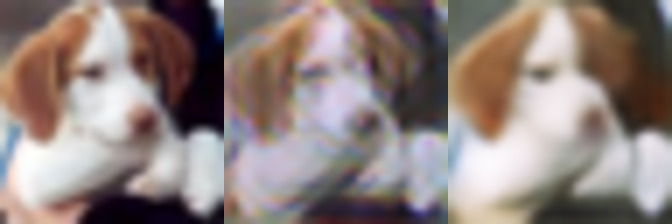
\includegraphics[width=0.63\textwidth]{figs/resnet28/rec_tile_5.jpg}


\includegraphics[width=0.63\textwidth]{figs/resnet28/rec_tile_1.jpg}


\includegraphics[width=0.63\textwidth]{figs/resnet28/rec_tile_2.jpg}
\end{center}
\captionof{figure}{\label{fig:inversion_resnet28} AR WideResNet-28-10 reconstruction on CIFAR-10.}
\end{minipage}
\vspace{-1 cm}
\end{table}



\subsection{Robustness Level vs. Reconstruction Accuracy}
\label{relationship_adversarial}
We complement the reconstruction analysis by exploring the relation between adversarial robustness and inversion quality. We train five AlexNet classifiers on ImageNet, one on natural images (standard) and four via $\ell_{2}$-PGD attacks with $\varepsilon\in \{0.5,2,3,4\}/255$. All other training parameters are identical across models.

For each classifier, an image generator is trained on an ImageNet subset via pixel, feature and GAN losses to invert \layer{conv5} features. Similar to \secref{sec:experimental_inverting}, all five generators correspond to the mirror network of the encoder. To realiably measure the impact of adversarial robustness, reconstruction accuracy is evaluated in terms of PSNR, SSIM and LPIPS. We also report the effective robustness level achieved by each model via AutoAttack (\tabref{tab:rob_vs_acc}).
\begin{table}[t]
\begin{center}
\vspace{0.3cm}
\caption{\label{tab:rob_vs_acc} Reconstruction vs. Robustness. Experiments on ImageNet show that learning to invert AlexNet features with different AR levels can significantly improve the reconstruction accuracy.}
\resizebox{0.75\columnwidth}{!}{
\begin{tabular}{c|c|c|c|c|c}
\specialrule{.15em}{.05em}{.05em}
& \multicolumn{5}{c}{$\ell_{2}$ PGD Attack ($\varepsilon$)}\\
\cline{2-6}
& $0$ & $0.5$ & $2$ & $3$ & $4$ \\
\hline
\makecell{Standard Accuracy} & $53.69$ & $49.9$ & $43.8$ & $39.83$ & $36.31$\\
\makecell{AutoAttack \cite{croce_2020_reliable}} & \makecell{$8.19$ ($\varepsilon=0.5$)} & \makecell{$48.0$ ($\varepsilon=0.5$)} & \makecell{$28.0$ ($\varepsilon=2$)} & \makecell{$22.27$ ($\varepsilon=3$)} & \makecell{$14.9$ ($\varepsilon=4$)}\\
\hline
PSNR (dB) $\uparrow$ & $13.12$ & $14.41$ & $15.5$ & ${15.53}$ & $\mathbf{15.61}$\\
SSIM $\uparrow$ & $0.20$ & $0.26$ & $\mathbf{0.3}$ & ${0.26}$ & $0.25$\\
LPIPS $\downarrow$ & $0.657$ & ${0.625}$ & $\mathbf{0.614}$ & $0.629$ & $0.644$\\
\specialrule{.15em}{.05em}{.05em} 
\end{tabular}}
\end{center}
\vspace{-0.5cm}
\end{table}

\begin{table}[t]
\centering
\setlength\tabcolsep{2pt}
\begin{minipage}{0.5\textwidth}
\begin{center}
\vspace{-0.8 cm}
\caption{\label{tab:eval_scale} Reconstructing upscaled ImageNet samples. Images upscaled by a factor $L$ are reconstructed from their standard and AR AlexNet features. In contrast to the degraded standard reconstructions, AR reconstructions show an outstanding accuracy that improves for large scaling factors.}
\vspace{0.1 cm}
\fontsize{8.5}{10.5}\selectfont
\def\arraystretch{1.25}
\resizebox{1\columnwidth}{!}{%
\begin{tabular}{c|c|c|c|c|c|c}
\specialrule{.15em}{.05em}{.05em} 
\multirow{2}{*}{\makecell{$L$}} & \multicolumn{3}{c|}{\makecell{Standard\\AlexNet}} & \multicolumn{3}{c}{\makecell{Robust\\AlexNet}} \\
\cline{2-7}
& \makecell{PSNR\\(dB)$\uparrow$} & SSIM$\uparrow$ & LPIPS$\downarrow$ & \makecell{PSNR\\(dB)$\uparrow$} & SSIM$\uparrow$ & LPIPS$\downarrow$\\
\hline
 $1$ & \makecell{$15.057$} & \makecell{$0.3067$} & \makecell{$0.5473$} & \makecell{$17.2273$} & \makecell{$0.3580$} & \makecell{$0.5665$}\\
 $4$ & \makecell{$15.4258$} & \makecell{$0.4655$} & \makecell{$0.4136$} & \makecell{$22.575$} & \makecell{$0.5892$} & \makecell{$0.4012$}\\
 $7$ & \makecell{$13.8922$} & \makecell{$0.4852$} & \makecell{$0.4587$} & \makecell{$23.5778$} & \makecell{$0.6588$} & \makecell{$0.3898$}\\
 $10$ & \makecell{$13.1013$} & \makecell{$0.4969$} & \makecell{$0.486$} & \makecell{$23.9566$} & \makecell{$0.7244$} & \makecell{$0.3892$}\\
\specialrule{.15em}{.05em}{.05em} 
\end{tabular}
}
\end{center}
\end{minipage}
\hfill
\begin{minipage}{0.475\textwidth}

\begin{minipage}{0.2\textwidth}
\centering\textbf{\colorbox{white}{\scalebox{0.68}{G. truth}}}
\end{minipage}\begin{minipage}{0.2\textwidth}
\centering \colorbox{white}{\scalebox{0.7}{$L= 1$}}
\end{minipage}\begin{minipage}{0.2\textwidth}
\centering \colorbox{white}{\scalebox{0.7}{$L= 4$}}
\end{minipage}\begin{minipage}{0.2\textwidth}
\centering \colorbox{white}{\scalebox{0.7}{$L= 7$}}
\end{minipage}\begin{minipage}{0.2\textwidth}
\centering \colorbox{white}{\scalebox{0.7}{$L= 10$}}
\end{minipage}

\vspace{-0.05 cm}
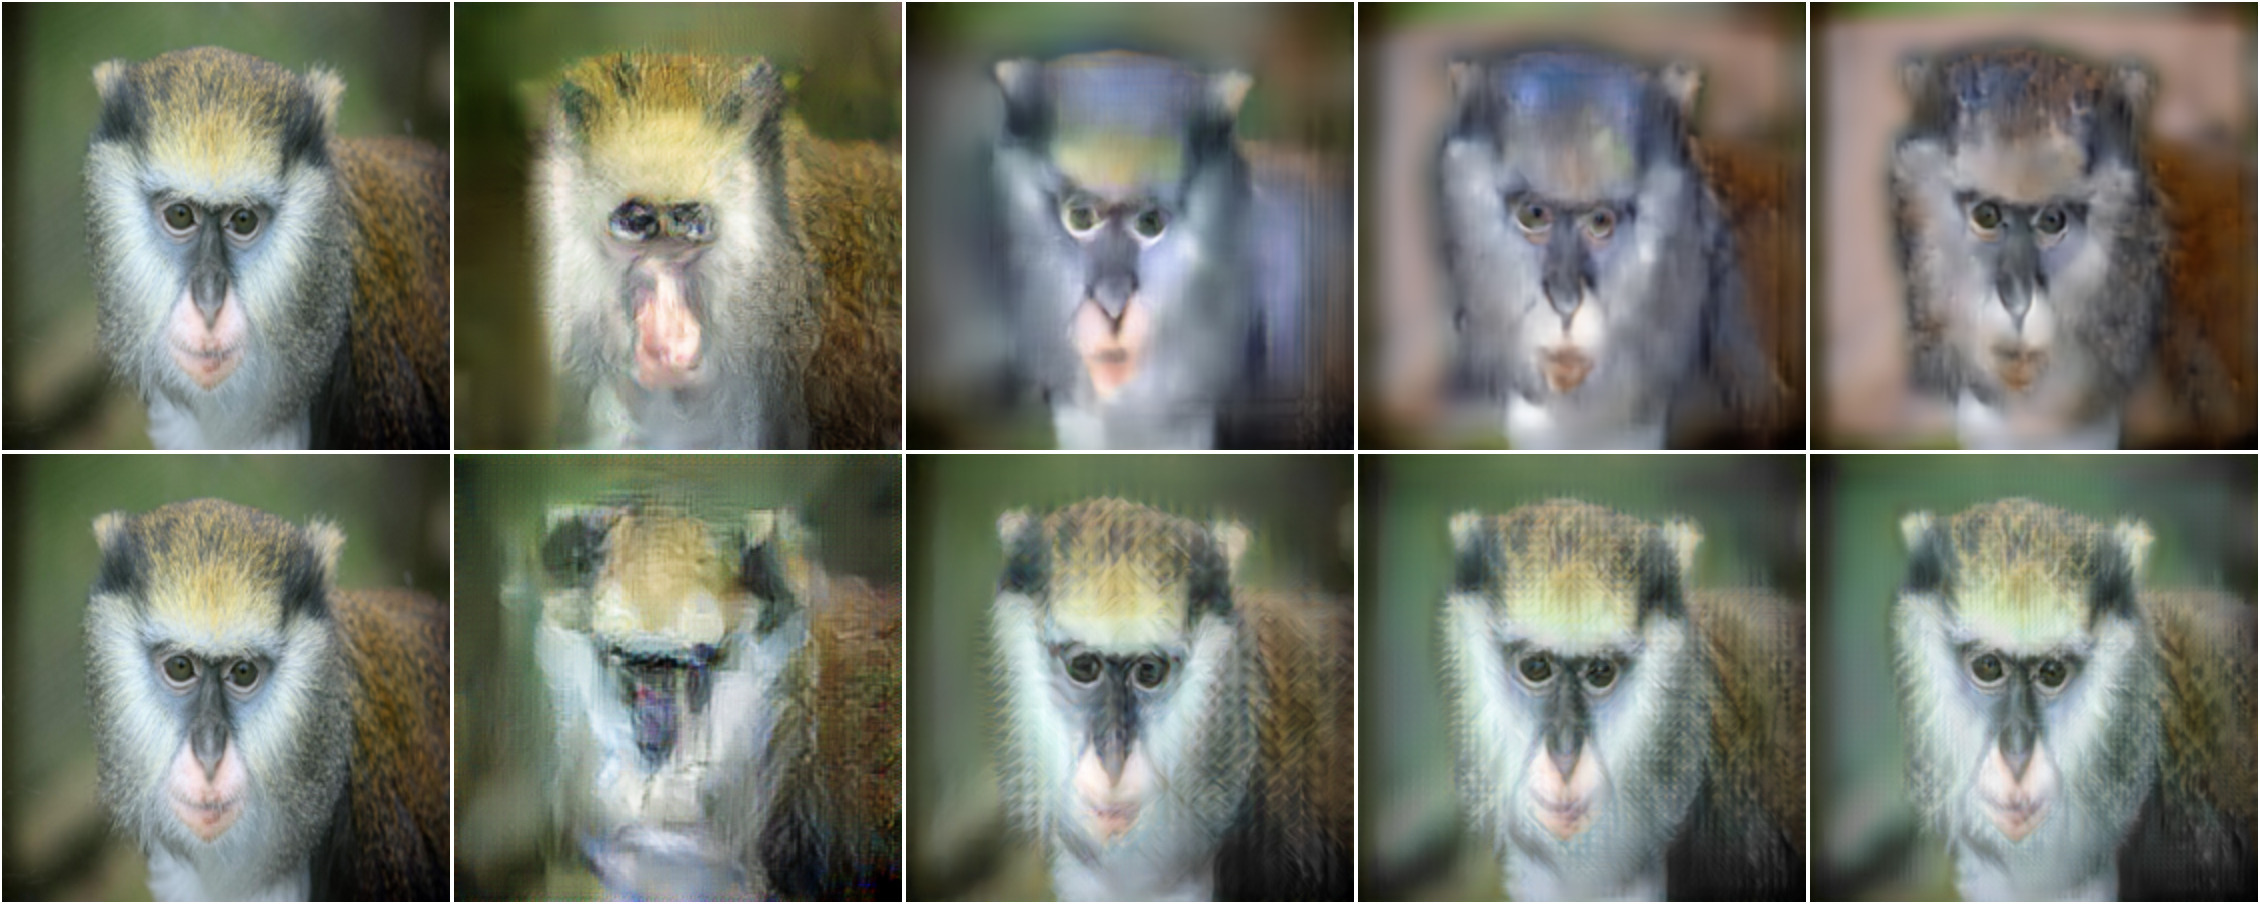
\includegraphics[width=1\textwidth]{figs/upscaling/tile_group_hires01_2.jpg}

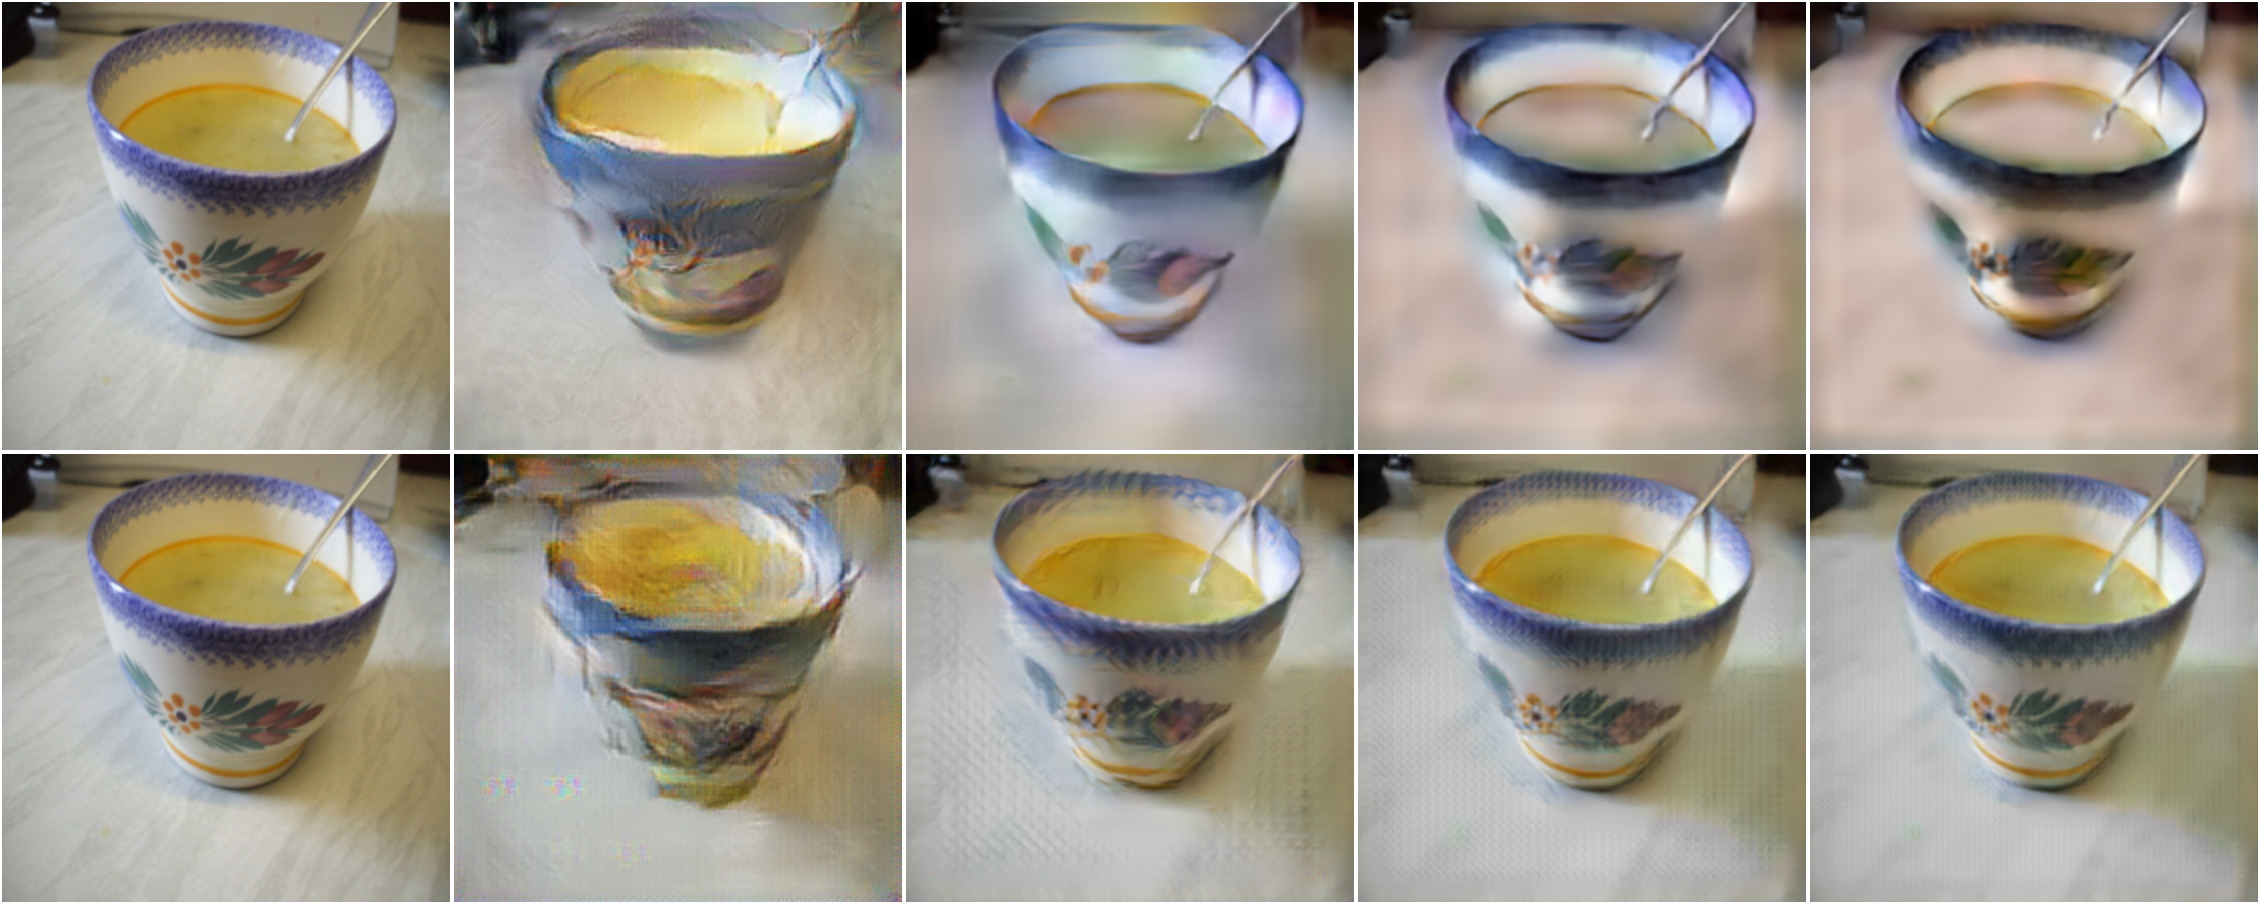
\includegraphics[width=1\textwidth]{figs/upscaling/tile_group_hires01_1.jpg}

\vspace{0.3 cm}
\captionof{figure}{\label{fig:eval_scale}Upscaled ImageNet samples reconstructed from their standard (top row) and AR (bottom row) features.}

\end{minipage}
\vspace{-0.5cm}
\end{table}


Results show LPIPS and SSIM improve almost monotonically until a maximum value is reached at $\varepsilon=2$, while PSNR keeps increasing. This implies that just by changing $\varepsilon$ from $0.5$ to $4$ while keeping the exact same architecture and training regime, a reconstruction improvement of $1.2$ dB PSNR is obtained.

Based on this, we use an AR AlexNet model trained with $\varepsilon=3$ in our experiments, which gives the best tradeoff between PSNR, SSIM and LPIPS. Overall, our analysis suggests that, while all four AR models outperform the inversion accuracy of the standard model, the reconstruction improvement is not proportional to the robustness level. Instead, it is maximized at a particular level. Please refer to \secref{sec:supp_inverting_alternative} for additional robustness level vs. reconstruction accuracy experiments on ResNet-18 pointing to the same conclusion.

\subsection{Reconstructing Images at Unseen Resolutions}
\label{sec:experimental_scale}

Unlike extracting shift-invariant representations, image scaling is difficult to handle for standard CNN-based models \cite{sosnovik_2019_scale,fan_2020_scale}. Following previous work suggesting AR features are more generic and transferable than standard ones \cite{chen2020shape,salman_2020_adversarially}, we test whether our proposed AR autoencoder generalizes better to scale changes. We explore this property and show that our model trained on low-resolution samples improves reconstruction of images at unseen scales without any fine-tuning.

\textbf{Scenario 1: Reconstructing Upscaled Images.} Upscaled ImageNet samples are reconstructed from their AR AlexNet \layer{conv5} representations. For a fair comparison across scales, each image is normalized to $224 \times 224$ px. and then enlarged by an integer factor $L>1$. Experiments show a higher accuracy obtained from AR features in terms of PSNR, SSIM and LPIPS (\tabref{tab:eval_scale}). All metrics improve almost monotonically with $L$. In contrast, accuracy using standard features degrades with $L$.
Inversion from AR features show almost perfect reconstruction for large scales, while those of standard features show severe distorsions (\figref{fig:eval_scale}).

\begin{table}[bpt!]
\begin{center}
\vspace{-0.2 cm}
\caption{\label{tab:hires} High-resolution images inverted using our AR AlexNet model (trained on low resolution images) show improved quality over standard inversions.}
\vspace{0.1 cm}
\fontsize{8.5}{10.5}\selectfont
\setlength\tabcolsep{2pt}
\resizebox{0.75\columnwidth}{!}{
\begin{tabular}{c|c|c|c} 
\specialrule{.15em}{.05em}{.05em} 
\makecell{Encoder} & PSNR (dB)$\uparrow$ & SSIM$\uparrow$ & LPIPS$\downarrow$\\
\hline
 Standard & \makecell{$14.266\pm$ $1.9015$} & \makecell{$0.3874\pm$ $0.151$} & \makecell{$0.5729\pm$ $0.0465$}\\
 AR (ours) & \makecell{$\mathbf{18.3606\pm}$ $\mathbf{2.6012}$} & \makecell{$\mathbf{0.4388\pm}$ $\mathbf{0.1508}$} & \makecell{$\mathbf{0.5673\pm}$ $\mathbf{0.0337}$}\\
\specialrule{.15em}{.05em}{.05em} 
\end{tabular}
}
\end{center}
\vspace{-0.625 cm}
\end{table}

\begin{figure}[t]
\begin{minipage}[t]{0.166\textwidth}
\centering\textbf{\colorbox{white}{\scalebox{.8}{Ground-truth}}}
\end{minipage}\begin{minipage}[t]{0.166\textwidth}
\centering \textbf{\colorbox{white}{\scalebox{.8}{Standard}}}
\end{minipage}\begin{minipage}[t]{0.1725\textwidth}
\centering \textbf{\colorbox{white}{\scalebox{.8}{AR (Ours)}}}
\end{minipage}\begin{minipage}[t]{0.166\textwidth}
\centering\textbf{\colorbox{white}{\scalebox{.8}{Ground-truth}}}
\end{minipage}\begin{minipage}[t]{0.166\textwidth}
\centering \textbf{\colorbox{white}{\scalebox{.8}{Standard}}}
\end{minipage}\begin{minipage}[t]{0.166\textwidth}
\centering \textbf{\colorbox{white}{\scalebox{.8}{AR (Ours)}}}
\end{minipage}

\vspace{-0.1 cm}    
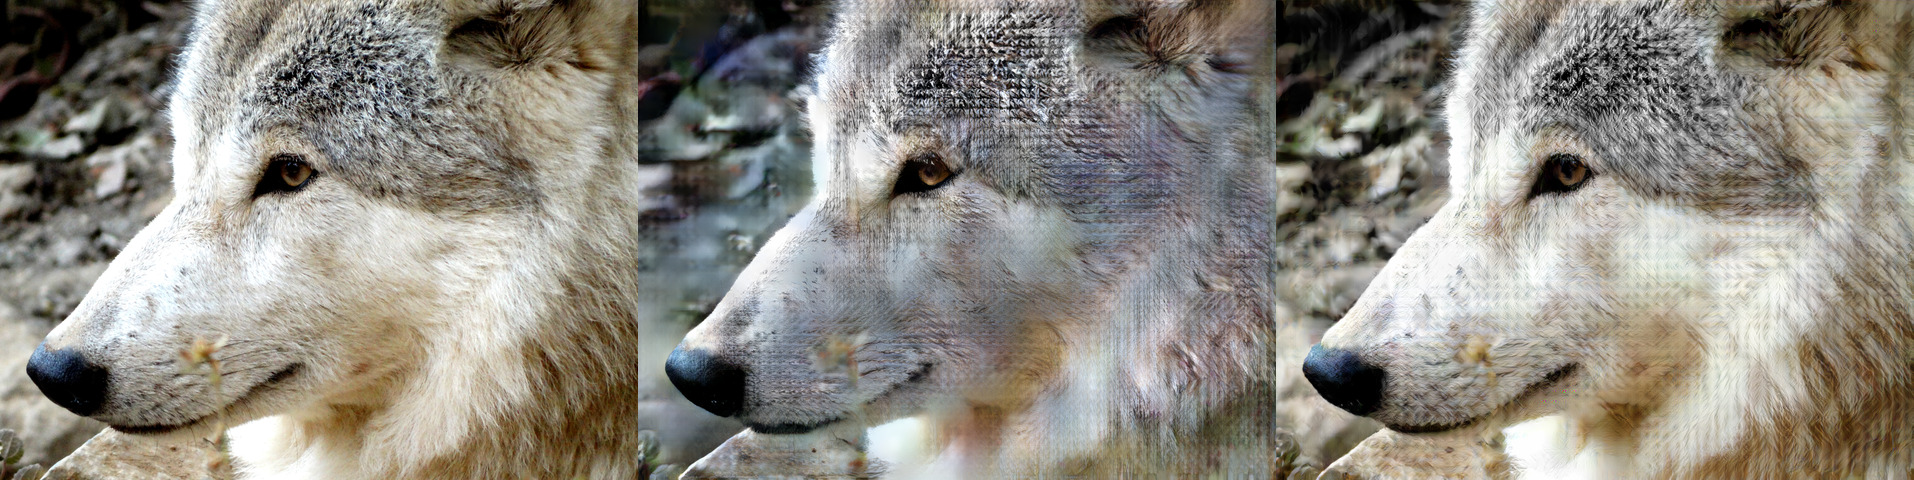
\includegraphics[width=0.5\textwidth]{figs/hires/tile_hires01_7.jpg}
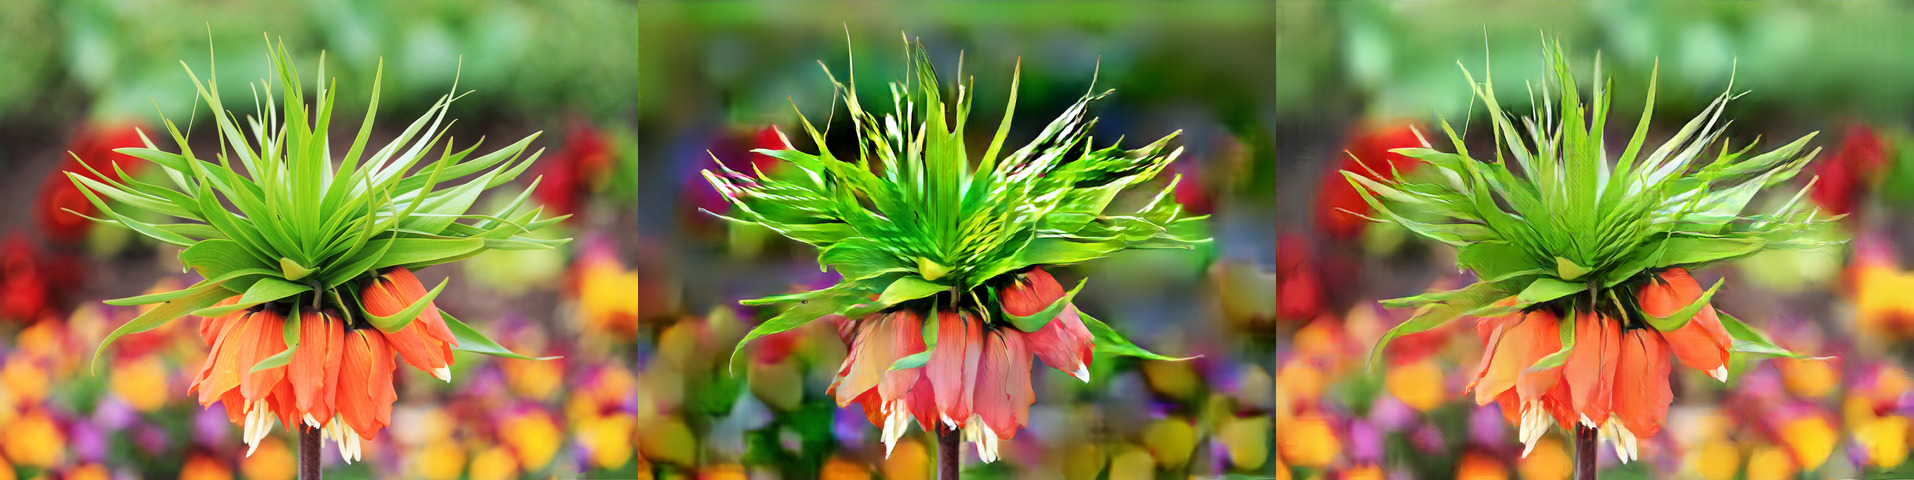
\includegraphics[width=0.5\textwidth]{figs/hires/tile_hires01_5.jpg}

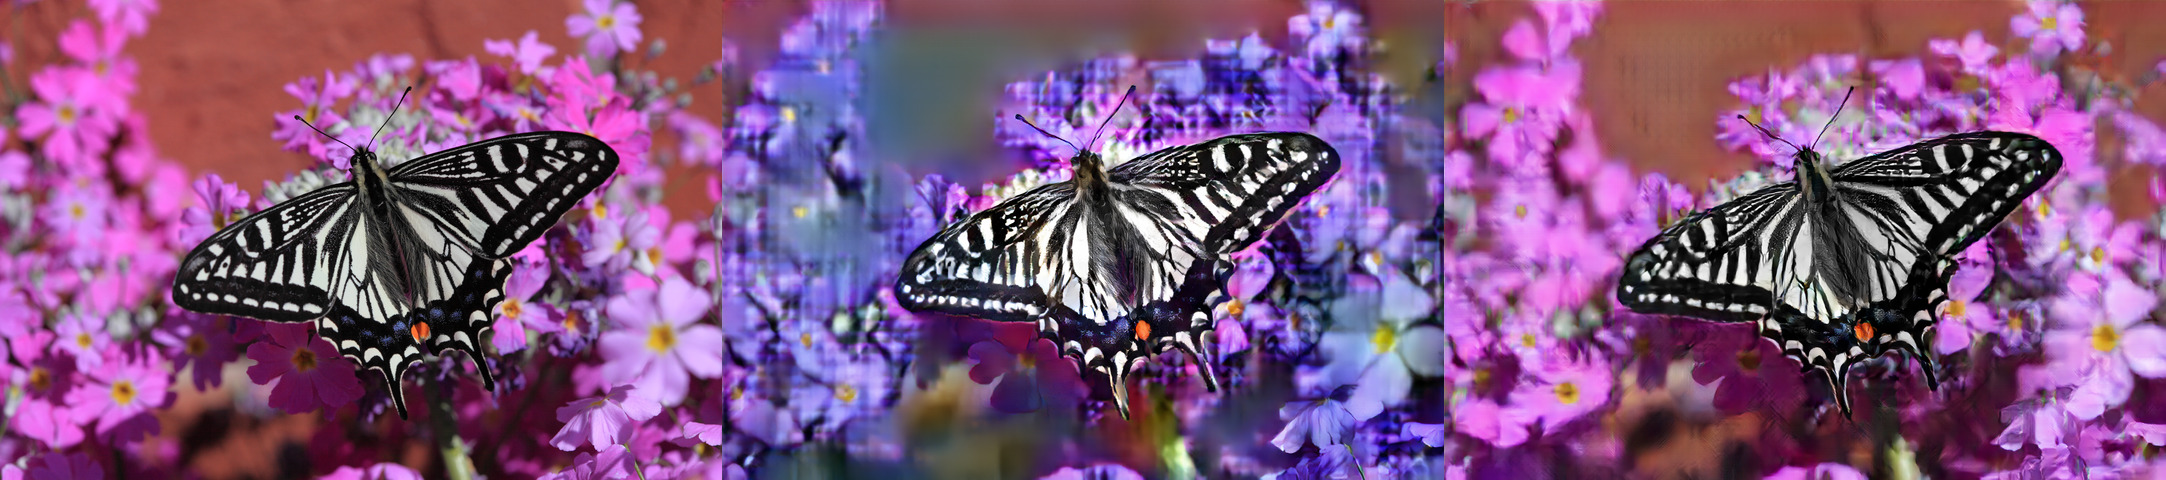
\includegraphics[width=0.5\textwidth]{figs/hires/tile_hires01_10.jpg}
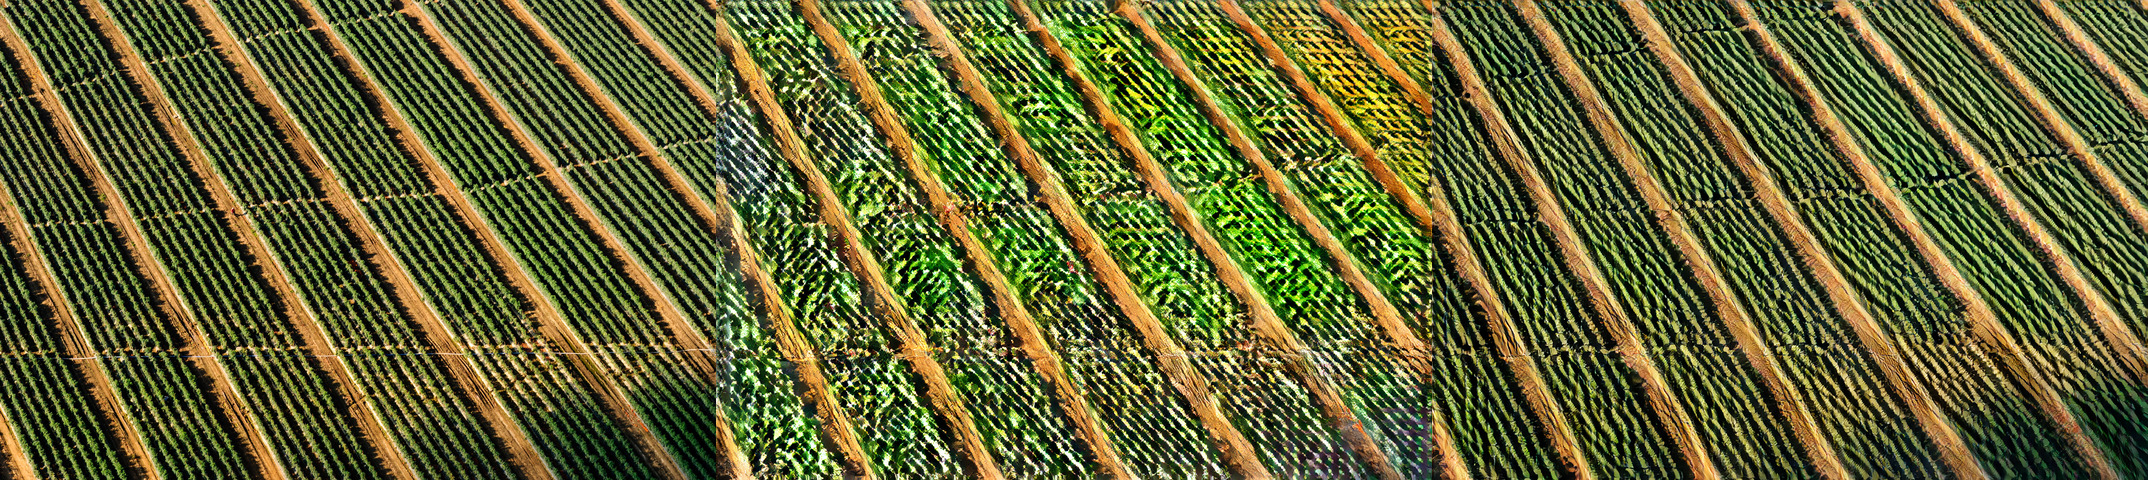
\includegraphics[width=0.5\textwidth]{figs/hires/tile_hires01_11.jpg}

\vspace{-0.1 cm}
\caption{\label{fig:hires}At a resolution of $2040\times 1536$ px., $10$ times larger than training samples, standard reconstructions on DIV2K show color and structure degradation. In contrast, reconstructions from our AR model do not suffer from distortions.}
\vspace{-0.5 cm}
\end{figure}


\textbf{Scenario 2: Reconstructing High-Resolution Images.} Standard and AR feature inversion is performed on the DIVerse 2K resolution dataset (DIV2K) \cite{agustsson_2017_ntire}, containing objects at multiple scales. AR feature reconstructions show a significant PSNR, SSIM and LPIPS improvement over standard ones, despite not being explicitly trained to handle such large-scale objects (\tabref{tab:hires}).

Qualitatively, reconstructions from AR AlexNet features preserve sharp edges, reduces color degradation and diminishes checkerboard effects induced by standard inversion (\figref{fig:hires}). Thus, for unseen scales and without finetuning, AR features better preserve structure without penalizing the perceptual similarity.

\subsection{Comparison against State-of-the-Art Inversion Techniques}
\label{sec:experimental_comparison}
The inversion accuracy of our AR autoencoder is compared against two alternative techniques: Optimization-based robust representation inversion (RI) \cite{engstrom_2019_adversarial} and DeePSiM \cite{dosovitskiy_2015_inverting}. For a fair comparison, all methods reconstruct images from AlexNet features. We begin by highlighting the differences between them.

While RI is a model-based approach that searches in the pixel domain for an image that matches a set of target AR features, we use a CNN-based generator trained on a combination of natural-image priors (\secref{sec:opt_crit}). On the other hand, while DeePSiM is also a CNN-based technique trained under multiple priors, its generator has approximately $63\%$ more trainable parameters than ours (\tabref{tab:inversion_comparison}).

\textbf{Experimental Setup.} All inversion methods are evaluated on ImageNet. Our standard and AR models are trained using pixel, feature and GAN losses using the training setup described in \secref{sec:supp_proposed_method}. DeePSiM is evaluated using its official Caffe implementation without any changes. RI is evaluated using its official PyTorch implementation modified to invert \layer{conv5} AR features. Input samples are rescaled to $224 \times 224$ px. ($227 \times 227$ px. for DeepSiM).

\textbf{Results.} Our AR AlexNet autoencoder obtains the best accuracy in terms of PSNR and the second best in terms of SSIM (\tabref{tab:inversion_comparison}). While it outperforms its standard version in PSNR and SSIM, it gets a marginally worse LPIPS. Moreover, our AR model outperforms RI in all metrics. Also, despite DeePSiM having more layers and using larger inputs, our model achieves a large PSNR improvement over it. Results highlight the improvement obtained by inverting AR features and how this fundamental change allows competitive reconstruction quality using three times less trainable parameters.

\begin{table}[t]
\centering
\vspace{-0.3cm}
\caption{\label{tab:inversion_comparison} Comparison against state-of-the-art inversion techniques. By inverting AR features, our autoencoder outperforms the optimization-based RI method by a large margin. Despite having 63\% less parameters, we also obtain favorable results against DeepSiM, showing a significant PSNR improvement.}%
\vspace{0.1 cm}
\resizebox{\columnwidth}{!}{

\begin{tabular}{c|c|c|c|c|c}
\specialrule{.15em}{.05em}{.05em} 
Algorithm & Encoder & Trainable Pars. & PSNR (dB)$\uparrow$ & SSIM$\uparrow$ & LPIPS$\downarrow$ \\
\hline
\makecell{RI \cite{engstrom_2019_adversarial}} & \makecell{AR AlexNet} & $-$ & $16.724\pm 2.434$ & $0.181\pm 0.071$ & $0.63\pm 0.04$\\
\makecell{Standard Autoencoder} & \makecell{Standard AlexNet} & $4,696,026$ & $15.057\pm 2.392$ & $0.307\pm 0.158$ & $\mathbf{0.547\pm 0.055}$\\
\makecell{AR Autoencoder (ours)} & \makecell{AR AlexNet} & $4,696,026$ & $\mathbf{17.227\pm 2.725}$ & $\mathbf{0.358\pm 0.163}$ & $0.567\pm 0.056$\\
\hline\hline
\makecell{DeepSiM \cite{dosovitskiy_2016_generating}} & \makecell{Standard CaffeNet} & $12,702,307$ & $15.321\pm 2.011$ & $0.417\pm 0.158$ & $0.531\pm 0.059$\\
\specialrule{.15em}{.05em}{.05em} 
\end{tabular}}
\vspace{-0.55 cm}
\end{table}

